\documentclass[10pt]{article}
%General Packages
\usepackage{multicol, enumerate, enumitem, hyperref, color, soul, setspace, parskip, fancyhdr}

%Math Packages
\usepackage{amssymb, amsthm, amsmath, bbm, latexsym, units, mathtools}

%All math in Display Style
\everymath{\displaystyle}

% Packages with additional options
\usepackage[T1]{fontenc}
\usepackage[headsep=0.5cm,headheight=0cm, left=1 in,right= 1 in,top= 1 in,bottom= 1 in]{geometry}
\usepackage[usenames,dvipsnames]{xcolor}

% SageTeX
\usepackage{sagetex}

% Package to use the command below to create lines between items
\usepackage{dashrule}
\newcommand{\litem}[1]{\item#1\hspace*{-1cm}\rule{\textwidth}{0.4pt}}

\pagestyle{fancy}
	\lhead{Module 6 - Polynomial Equations}
	\chead{}
	\rhead{Progress Exam 3}
	\lfoot{Spring 2019}
	\cfoot{}
	\rfoot{Version A}

\begin{document}
	\pagestyle{fancy}

\begin{sagesilent} 
load("../Code/generalPurposeMethods.sage")
load("../Code/keyGeneration.sage")
\end{sagesilent}

\begin{enumerate}
\setcounter{enumi}{25}
%OBJECTIVE 1 - Convert between a polynomial function and its graph.
\begin{sagesilent}
version = "A"
moduleNumber = 6
problemNumber = 26
load("../Code/polynomial/polyGraphToFunction.sage")
\end{sagesilent}
% TYPE 1 - Function to graph

% TYPE 2 - Graph to function 
\litem{ \sage{displayStem}
	\begin{center}
	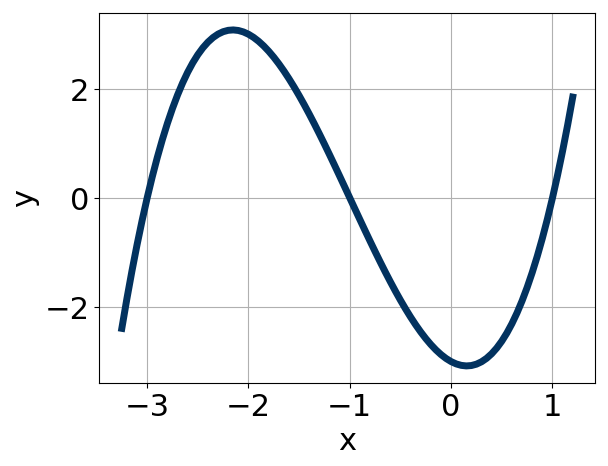
\includegraphics[width = 0.5\textwidth]{../Figures/question26A.png}
	\end{center}
	\begin{enumerate}[label=\Alph*.]
		\item $\sage{choices[0]}$
		\item $\sage{choices[1]}$
		\item $\sage{choices[2]}$
		\item $\sage{choices[3]}$
		\item $\sage{choices[4]}$
	\end{enumerate}	
}
	
%OBJECTIVE 2 - Indetify the end behavior and zero behavior of a polynomial equation
\begin{sagesilent}
problemNumber = 27
load("../Code/polynomial/polyEndAndZeroBehavior.sage")
\end{sagesilent}
%TYPE 1 - End behavior
\litem{ \sage{displayStem1}
	$$f(x) = \sage{displayPolynomial} $$
\begin{multicols}{2}
	\begin{enumerate}[label=\Alph*.]
		\item \begin{center} 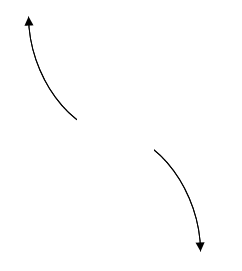
\includegraphics[scale=0.5]{endBehaviorNegativeOdd} \end{center}
		\item \begin{center} 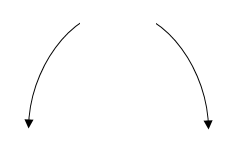
\includegraphics[scale=0.5]{endBehaviorNegativeEven}\end{center}
		\item \begin{center} 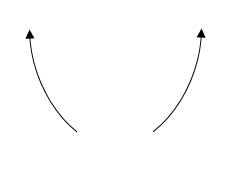
\includegraphics[scale=0.5]{endBehaviorPositiveEven}\end{center}
		\item \begin{center} 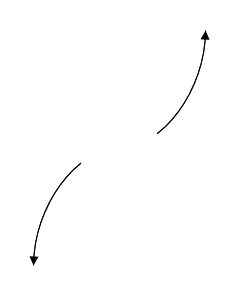
\includegraphics[scale=0.5]{endBehaviorPositiveOdd}\end{center}
	\end{enumerate}	
\end{multicols}
}

\newpage

%TYPE 2 - Zero behavior
\litem{Describe the zero behavior of the zero $\sage{zeroOnDisplay}$ of the polynomial below.
	$$f(x) = \sage{displayPolynomial} $$
\begin{multicols}{2}
	\begin{enumerate}[label=\Alph*.]
		\item \begin{center} 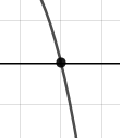
\includegraphics[scale=0.7]{zeroBehaviorNegativeOdd}\end{center}
		\item \begin{center} 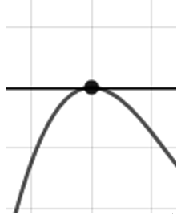
\includegraphics[scale=0.5]{zeroBehaviorNegativeEven}\end{center}
		\item \begin{center} 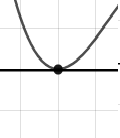
\includegraphics[scale=0.7]{zeroBehaviorPositiveEven}\end{center}
		\item \begin{center} 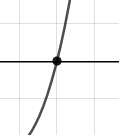
\includegraphics[scale=0.7]{zeroBehaviorPositiveOdd}\end{center}
	\end{enumerate}	
\end{multicols}
}

%OBJECTIVE 3 - Construct lowest-degree polynomials given the zeros of the polynomial.
\begin{sagesilent}
problemNumber = 29
load("../Code/polynomial/constructPolyRationals.sage")
\end{sagesilent}
% TYPE 1 - Construct with all rational zeros.
\litem{ \sage{displayStem}
	$$ \sage{displayZero1}, \sage{displayZero2}, \sage{displayZero3} $$
	\begin{enumerate}[label=\Alph*.]
		\item $\sage{choices[0]}$
		\item $\sage{choices[1]}$
		\item $\sage{choices[2]}$
		\item $\sage{choices[3]}$
		\item $\sage{choices[4]}$
	\end{enumerate}	\vspace*{-4mm}
}

\begin{sagesilent}
problemNumber = 30
load("../Code/polynomial/constructPolyComplex.sage")
\end{sagesilent}

% TYPE 2 - Construct with irrational or complex roots.
\litem{ \sage{displayStem}
	$$ \sage{displayZero1} \text{ and } \sage{displayZero2}$$
	\begin{enumerate}[label=\Alph*.]
		\item $\sage{choices[0]}$
		\item $\sage{choices[1]}$
		\item $\sage{choices[2]}$
		\item $\sage{choices[3]}$
		\item $\sage{choices[4]}$
	\end{enumerate}	\vspace*{-4mm}
}

\end{enumerate}

\end{document}